%% The first command in your LaTeX source must be the \documentclass command.
\documentclass[acmconf]{acmart}
% % Packages
%\usepackage{cite}
\usepackage{listings}
\usepackage{amsmath,amssymb,amsfonts}
\usepackage{algorithmic}
\usepackage{graphicx}
\usepackage{textcomp}
\usepackage{xcolor}
\usepackage{booktabs}
\usepackage{parskip}
\setlength{\parskip}{1em}
\usepackage[bottom]{footmisc}
\usepackage{enumitem}
\usepackage{hyperref}
\usepackage{totpages}
\usepackage{subfigure}

%% \BibTeX command to typeset BibTeX logo in the docs
\AtBeginDocument{%
  \providecommand\BibTeX{{%
    \normalfont B\kern-0.5em{\scshape i\kern-0.25em b}\kern-0.8em\TeX}}}

%% Rights management information.  This information is sent to you
%% when you complete the rights form.  These commands have SAMPLE
%% values in them; it is your responsibility as an author to replace
%% the commands and values with those provided to you when you
%% complete the rights form.
% \setcopyright{acmcopyright}
% \copyrightyear{2018}
% \acmYear{2018}
% \acmDOI{10.1145/1122445.1122456}

% %% These commands are for a PROCEEDINGS abstract or paper.
% \acmConference[Woodstock '18]{Woodstock '18: ACM Symposium on Neural
%   Gaze Detection}{June 03--05, 2018}{Woodstock, NY}
% \acmBooktitle{Woodstock '18: ACM Symposium on Neural Gaze Detection,
%   June 03--05, 2018, Woodstock, NY}
% \acmPrice{15.00}
% \acmISBN{978-1-4503-XXXX-X/18/06}



%%
%% The majority of ACM publications use numbered citations and
%% references.  The command \citestyle{authoryear} switches to the
%% "author year" style.
%%
%% If you are preparing content for an event
%% sponsored by ACM SIGGRAPH, you must use the "author year" style of
%% citations and references.
%% Uncommenting
%% the next command will enable that style.
%%\citestyle{acmauthoryear}

%%
%% end of the preamble, start of the body of the document source.
\begin{document}

% Specify path to images
\graphicspath{ {./img/} }

% import custom commands found in commands.tex
\newcommand{\fix}[1]{\textcolor{red}{#1}}
\newcommand{\derek}[1] {\textcolor{blue}{\textbf{[Derek: #1]}}}
\newcommand{\neha}[1] {\textcolor{green}{\textbf{[Neha: #1]}}}
\newcommand{\keanu}[1] {\textcolor{orange}{\textbf{[Keanu: #1]}}}
\newcommand{\manish}[1] {\textcolor{cyan}{\textbf{[Manish: #1]}}}
% set up commands to format RQ nicely
\newlist{questions}{enumerate}{2}
\setlist[questions,1]{label=RQ\arabic*.,ref=RQ\arabic*}
\setlist[questions,2]{label=(\alph*),ref=\thequestionsi(\alph*)}

%%
%% The "title" command has an optional parameter,
%% allowing the author to define a "short title" to be used in page headers.
\title[Survival Analysis of Open Source Projects]{Two Differing Approaches to Survival Analysis of Open Source Python Projects}

%%
%% The "author" command and its associated commands are used to define
%% the authors and their affiliations.
\author{Derek Robinson}
\email{drobinson@uvic.ca}
\author{Keanelek Enns}
\email{keanelekenns@uvic.ca}
\author{Neha Koulecar}
\email{nehakoulecar@uvic.ca}
\author{Manish Sihag}
\email{manishsihag@uvic.ca}
\affiliation{%
  \institution{\\University of Victoria}
  \department{Computer Science}
  \streetaddress{PO Box 1700 STN CSC}
  \city{Victoria}
  \state{British Columbia}
  \country{Canada}
  \postcode{V8W 2Y2}
}

%%
%% By default, the full list of authors will be used in the page
%% headers. Often, this list is too long, and will overlap
%% other information printed in the page headers. This command allows
%% the author to define a more concise list
%% of authors' names for this purpose.
\renewcommand{\shortauthors}{D. Robinson, K. Enns, N. Koulecar, M. Sihag}

%%
%% The abstract is a short summary of the work to be presented in the
%% article.
\begin{abstract}
\keanu{Abstract Pending}
\end{abstract}

%%
%% The code below is generated by the tool at http://dl.acm.org/ccs.cfm.
%%
\begin{CCSXML}
<ccs2012>
<concept>
<concept_id>10011007.10011074.10011134.10003559</concept_id>
<concept_desc>Software and its engineering~Open source model</concept_desc>
<concept_significance>500</concept_significance>
</concept>
<concept>
<concept_id>10002951.10003227.10003351</concept_id>
<concept_desc>Information systems~Data mining</concept_desc>
<concept_significance>300</concept_significance>
</concept>
</ccs2012>
\end{CCSXML}

\ccsdesc[500]{Software and its engineering~Open source model}
\ccsdesc[300]{Information systems~Data mining}

%%
%% Keywords. The author(s) should pick words that accurately describe
%% the work being presented. Separate the keywords with commas.
\keywords{data science, survival analysis, open source, python, Kaplan Meier, Cox proportional hazards model, Bayesian analysis}


%%
%% This command processes the author and affiliation and title
%% information and builds the first part of the formatted document.
\maketitle

\section{Introduction} \label{intro}
The developers of Open Source Software (OSS) projects are often part of decentralized and geographically distributed teams of volunteers.
As these developers volunteer their free time to build such OSS projects, they likely want to be confident that the projects they work on will not become inactive.
If OSS developers are aware of key attributes that are associated with long-lasting projects, they can make informed assessments of a given project before devoting their time to it or they can strive to make their own projects exhibit those attributes.
Understanding which attributes of an OSS project lead to its longevity is what motivated Ali \emph{et al.} to apply survival analysis techniques commonly found in biostatistics to study the probability of survival for popular OSS Python projects \cite{ali2020cheating}.
Ali \emph{et al.} specifically studied the effect of the following attributes on the survival of OSS Python projects: publishing major releases, the use of multiple hosting services, the type of version control system (VCS), and the size of the volunteer team.

Survival analysis is a set of methods used to determine how long an entity will live (or the time to a given event) and is most often used in the medical field.
For example, survival analysis techniques can determine the probability that a patient will survive past a certain time when given a certain treatment. 
Ali \emph{et al.} use a frequentist approach to survival analysis utilizing such methods as the Kaplan-Meier (K-M) survival estimator and the Cox Proportional-Hazards model \cite{kaplan1958nonparametric, cox1972regression}.
Though there are advantages to using such approaches \keanu{list some advantages and cite}, another approach to survival analysis, Bayesian analysis, has its own set of advantages. \keanu{find the advantages, list them, cite}.

The authors of this paper resonate with Ali \emph{et al.'s} motivation. 
This paper serves as a replication of their paper \cite{ali2020cheating} (referred to as the original paper from here on)  and seeks to determine if there are gaps or shortcomings in their analysis.
This replication also provides artifacts so that others may see how the study was conducted and reproduce it with ease.
For the sake of the authors' curiosity, an additional attribute of the data was analyzed: the commit frequency of the project.
In addition to the replication, this paper analyzes the same data set using a Bayesian approach to survival analysis as outlined in \cite{kelter2020bayesian} and seeks to compare the results of the frequentist and Bayesian approaches in the same domain.
Thus, the research questions this paper answers are as follows:

\begin{questions}
    \item How do major releases, the use of multiple hosting services, the type of VCS, and the size of the volunteer team affect the probability of survival of an OSS Python project?
    \item How does the commit frequency of an OSS Python project affect the probability of it's survival?
    \item How do the findings of frequentist survival analysis differ from Bayesian survival analysis?
\end{questions}

The following section describes the data used for the studies in this paper as well as the process used for manipulating the data into a usable state.
Section \ref{methods} covers the methods used for the replication, additional frequentist analysis, and Bayesian analysis.
Section \ref{results} shows the results for each analysis.
Section \ref{discussion} is a discussion about the comparative differences between the analyses performed, the limitations of the study, related work, and suggestions for future work in the topic.
The final section concludes by summarizing the purpose and findings of this paper. 

\section{Data} \label{data}

Performing survival analysis of OSS projects requires a data set that records the repositories for projects on common VCSs, including a history of all commits (revisions from here on out) and major releases (revisions of note, often with a specific name and release date) \cite{ali2020cheating}.
Revisions are used to assess the activity or health of a project.

The \emph{popular-3k-python} subset of the Software Heritage graph data set \cite{pietri2019software} contains the necessary information and was used in both the original paper and this paper (a reference to the data set can be found in appendix \ref{artifacts} of this paper).
This data set contains information on roughly 3000 popular Python projects hosted on GitHub/GitLab, Debian, and PyPI between 2005 and 2018.
The Software Heritage organization offers a tutorial on how to import this data by creating a postgreSQL database \cite{SQLdataset} as well as an explanation of the structure of the database (a database schema can be seen in figure 2 of their document \cite{pietri2019software}) .

Though the data contains all the necessary information to perform survival analysis on, it requires additional manipulation into a new format before the analysis can be carried out. 
For example, most of the analyzed features or attributes of the projects in the original paper are not present in the raw data set and need to be calculated.
The work done in this study has been documented in a repository for the benefit of the reader.
References to the repository can be found in appendix \ref{artifacts} and the jupyter notebook used to perform the data manipulation can be found in Analysis\&Data/data-collection.ipynb.

Queries were created in order to join the necessary tables and extract the relevant values.
The queries accomplish the following objectives: they group records by the \emph{url} field of the origin table (used to identify projects), filter records to be within the desired time frame, count distinct authors that have participated in a given project, record the host service (depicted by the \emph{type} field of the origin table), record the earliest and latest revisions associated with each project url, count the number of revisions made during each project's duration, and identify whether major releases were published.
\keanu{should we show pseudocode of one of the queries? Also, I wonder if we can find a way to condense the queries into as few queries as possible for the final product}
\derek{I think that condensing the queries is not required. If Neil decides to look at them he should be able to understand what is going on. If anything we should add explanatory markdown to the notebook.}

The notebook uses popular python libraries such as psycopg2, pandas, numpy, and matplotlib to connect to the database, extract the results of the previously mentioned queries, manipulate and filter the data, calculate new fields, and plot results.
\keanu{This section is getting long, I was going to go into details about the new fields that were calculated (multi\_repo, commit\_freq, etc.), but maybe we should wait and see}

% If we want filler we can add the schema diagram and talk about it.
% \begin{figure}[h]
% \centering
% 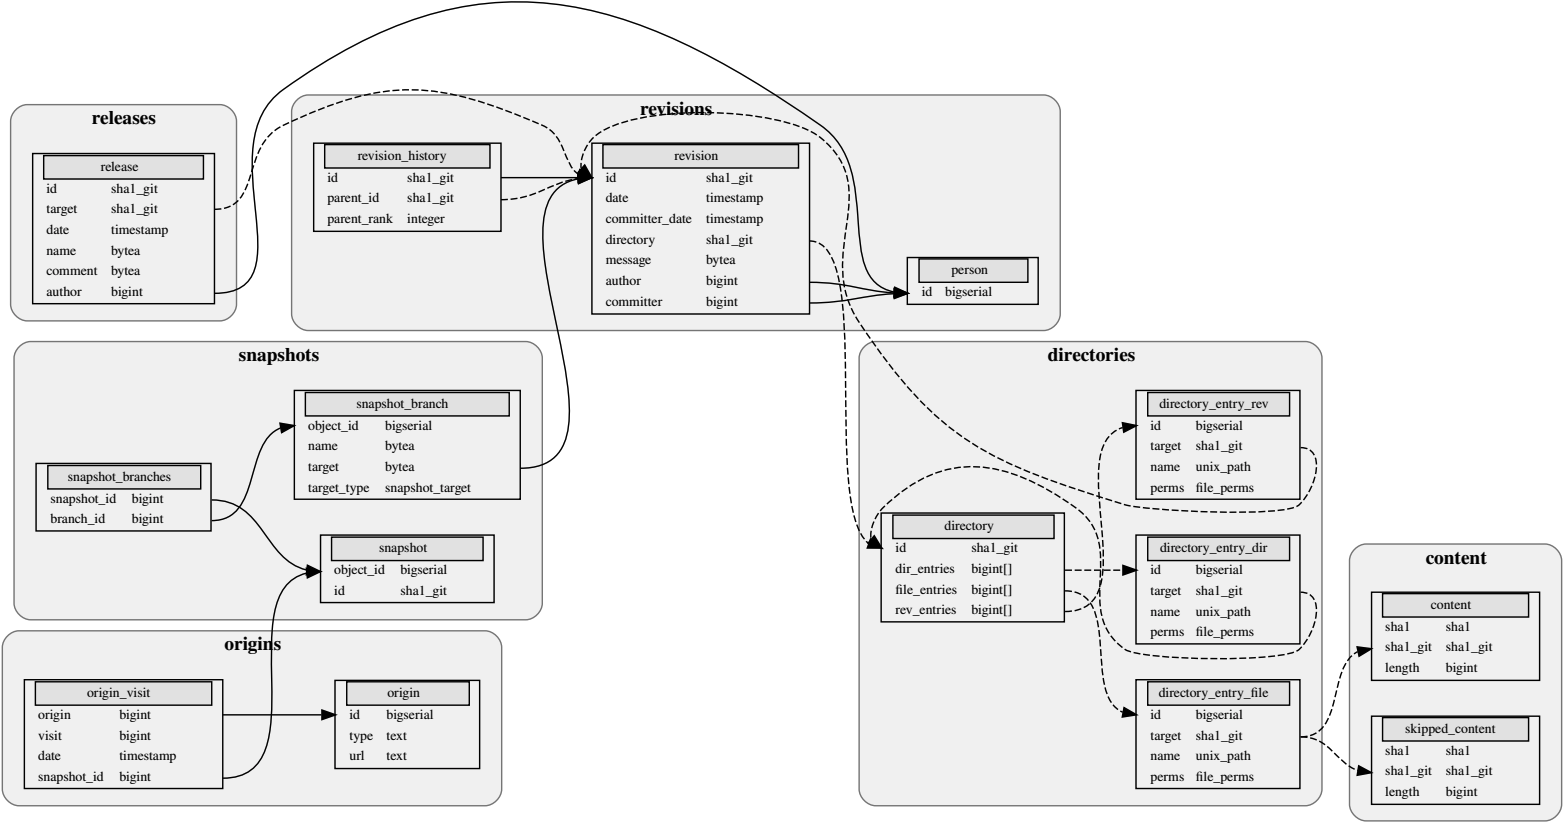
\includegraphics[scale=0.25]{dataset-schema.png}
% \Description{}
% \caption{The results of running the Cox Proportional hazards tool on the data. \keanu{we definitely want better descriptions for the images} \derek{I don't think that we really need the schema in the paper}}
% \label{fig:Schema}
% \end{figure}

\section{Methods} \label{methods}

\subsection{Replication}

Two critical concepts in survival analysis are events of interest and censoring.
In the case of this paper, as well as the original paper, the event of interest is the abandonment of a project.
That is, if a project stops receiving revisions, it is considered abandoned.
However, it is impossible to determine whether a project will receive revisions in the future, so a threshold of some kind is required to determine whether the project has indeed been abandoned for the purposes of the study.
This is where censoring is used.
Censoring involves using data from subjects of a study for which the time of interest is not observed.
There are multiple types of censoring in survival analysis, but this study uses random censoring or type III censoring \keanu{or right censoring, we should flesh out the terminology as I have seen some conflicting definitions}. \derek{I would say just go with that Ali et al. say (type III/random censoring)}
Random censoring involves removing subjects (in this case projects) from a study at varying times relative to when they began being observed \cite{renganathan2016overview}. \keanu{find another citation to support this, http://www.stat.columbia.edu/~madigan/W2025/notes/survival.pdf mentions it, but refer to it as random type 1 right censoring}

Ali \emph{et al.} set a time frame of 165 months (where a month is defined as 28 days), starting in 2005 and ending in January 2018.
This paper uses the same time frame and determines exact start and end dates.
Using January 1, 2018 as a strict end date and maintaining the study duration as 4620 days (165 months as defined), the start date is found to be May 9, 2005.

Projects are censored if there is reason to believe that they would receive revisions after the end of the time frame (i.e. the last \emph{observed} revision is unlikely to be the last revision of the project).
In this paper, any project with revisions on or after November 1, 2017 were censored. 
\keanu{NOTE: Our censoring method may change. This is because the paper \cite{ali2020cheating} conflicted with the video presentation \cite{ali2020video} with respect to the censoring method. After further inspection, it appears the method in the paper is superior, as we only censor data that truly had revisions after the time frame (though this probably will not affect many of the data points)}
The reason this is considered random censoring is because projects that are censored have varying start dates within the time frame of the study.
The distribution of the project timeline can be seen in Figure \ref{fig:figure-1} which is a replication of Figure 1 in the original paper.

\begin{figure}[ht]
\centering
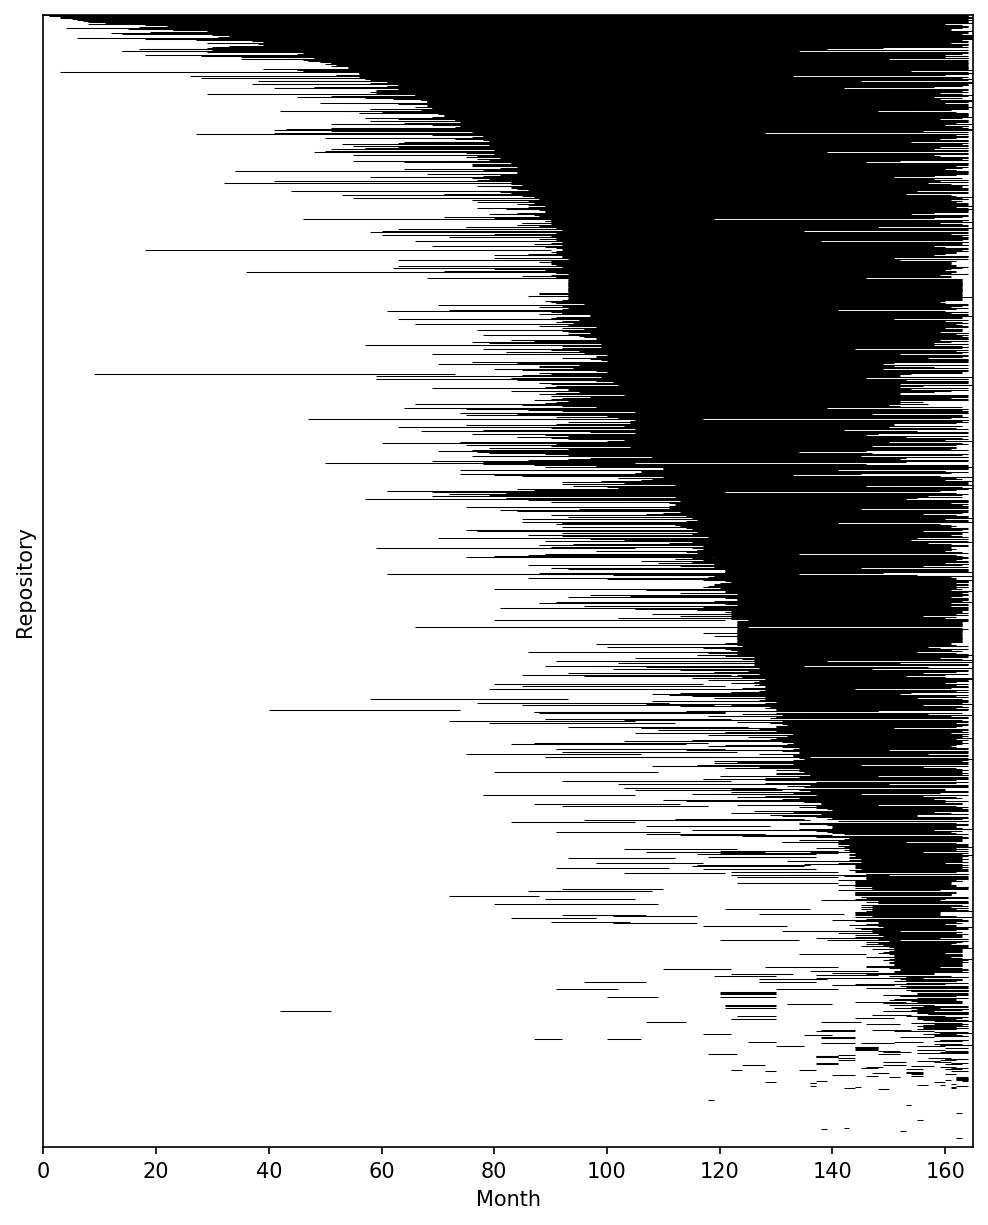
\includegraphics[scale=0.5]{figure1.jpg}
\caption{Graph of project timelines within the given time frame. The projects are ordered by duration and plotted from and to their respective beginning and ending dates.}
\label{fig:figure-1}
\end{figure}

Using both the calculated duration associated with each project and censoring status of each project, the survival analysis can be performed.
The analysis was carried out using an R notebook (this can be found in the repository under Analysis\&Data/KM-estimation.rmd \keanu{should probably change R notebook name to include Cox, maybe just frequentist-analysis.rmd?}).

\keanu{Manish, I need your help here because you know best how to explain what you did. For example, I am not sure how/if you used these references \cite{survivalRpackage, stel2011cox, stel2011kaplan}}

The K-M estimator is a non-parametric estimation technique that allows us to estimate the survival function, $S(t)$. 
The survival function is the probability that a given project will survive past a particular time $t$.  
At $t = 0$, the K-M estimator is 1 and as $t$ approaches infinity, so does the K-M estimator.
More precisely, $S(t)$ is given by  $S(t) = p_1 \times p_2 \times \dots \times p_t$, while $p_1$ is the proportion of all projects which survived at the first time point, similarly, $p_2$ is the proportion of all projects which survived at the second time point. 
The K-M estimator produces curves which approach the true survival function of the data.

\derek{This next sentence reads really weird but I am unsure how to reword it}
Another useful function in survival analyses is the hazard function, which describe the probability of an event or its hazard (survival in this case) of the project surviving up to that particular time point.
We are using the Cox proportional-Hazards model which allows us to fit a regression model in order to better understand how the health of projects relates to their key attributes. 
In the previously mentioned R notebook, we make use of the \lstinline[language=R]!survival! package for K-M estimation and Cox proportional-Hazards model. Additionally, we make use of the \lstinline[language=R]!survminer! package which provides functions for facilitating survival analysis and visualization. 
The analysis begins by using the \lstinline[language=R]!Surv()! method to build the standard survival object and the \lstinline[language=R]!survfit()! method to produce the K-M estimates of the probability of survival over time. K-M curves with their associated confidence interval for all the four attributes described in the original paper are generated via the \lstinline[language=R]!ggsurvplot()! function which, in addition, plots the p-value of a log rank test. 
The next step is to build the Cox proportional hazards using \lstinline[language=R]!coxph()! function and visualize them using the \lstinline[language=R]!ggforest!. 
This analysis results in the hazards ratio (HR) which is derived from the model for all covariates that we included in the formula. 
Briefly, a $HR > 1$ indicates an increased risk of death, on the other hand, $HR < 1$, indicates a decreased risk of death. 
As such, the HR represents a relative risk of death that compares one instance of a binary feature (eg. yes or no) to the other instance.

% From proposal:
% The K-M estimator is used to estimate the survival function. In our use case, the K-M estimator will estimate the probability that the duration of a project is longer than time $t$. The other analysis we will be performing is fitting a Cox Proportional-Hazards model. The Cox Proportional-Hazards model is a regression model that will allow us to investigate the association between the survival of a project and its key attributes.
\subsection{Revision Frequency Analysis}

The original paper mentions that ''The health of a project could be computed by the number and frequency of contributions...'', but never addresses this measurement.
This paper seeks to explore this method of assessment. 
We dichotomized the commit frequency into two groups depending on the frequency above and below the median. 
We apply both the K-M estimator to and the Cox Proportional-Hazards model on the data to stratify the effects of high commit frequency on the overall health of an open source project.

\subsection{Bayesian Survival Analysis}

This section focuses on the Bayesian approach to survival analysis as outlined in \cite{kelter2020bayesian}. 
Although applying the Bayesian approach to survival analysis is less common due to computational difficulties, it offers multiple advantages over the frequentist approach. 
The Bayesian analysis uses posterior distributions of model parameters to conclude them. 
These posterior distributions are obtained via Markov-Chain-Monte-Carlo (MCMC) algorithms. 
The statistical modelling language used for Bayesian analysis is Stan, specifically the \lstinline!rstan! interface. In addition to \lstinline!rstan!, the R packages \lstinline[language=R]!tidybayes! and \lstinline[language=R]!tidyverse! were used to aid in visualization and data manipulation.

We have used a parametric exponential model that assumes the survival times of a project $y = (y1, y2, \dots , yn)$ are exponentially distributed with parameter $\lambda$.
We have so far derived a posterior survival function for one of the project's attributes: the use of multiple VCSs. 
We will be further deriving posterior survival functions for the remaining attributes, namely major releases, VCS of the project, commit frequency and author count. 

% From proposal (slightly revised to make sense in this context):
% [This paper applies] the same methods as found in the section titled \emph{A detailed example} of \cite{kelter2020bayesian}. A parametric exponential model that assumes the survival times of a project $y = (y_1, y_2, \dots, y_n)$ are exponentially distributed with parameter $\lambda$ was created. This model was then used to visualize the posterior survival functions for the following five project attributes: major releases, VCS of the project, use of multiple VCSs, team size, and revision frequency.
\section{Results} \label{results}

\subsection{Replication}

We found the results of our replication study to be extremely similar to those shown in the original paper.

\begin{figure*}[ht]
    \centering
    \begin{subfigure}
        \centering
        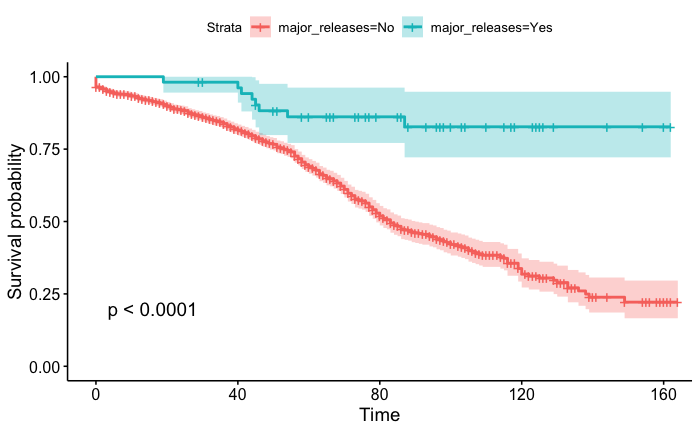
\includegraphics[width=0.45\textwidth]{major-releases.png}   
        \label{fig:major releases}
    \end{subfigure}
    \begin{subfigure}
        \centering 
        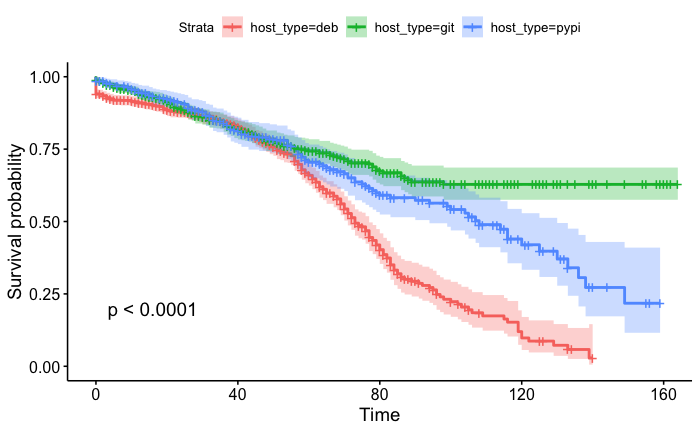
\includegraphics[width=0.45\textwidth]{host_type.png}
        \label{fig:host type}
    \end{subfigure}
    \vskip\baselineskip
    \begin{subfigure} 
        \centering 
        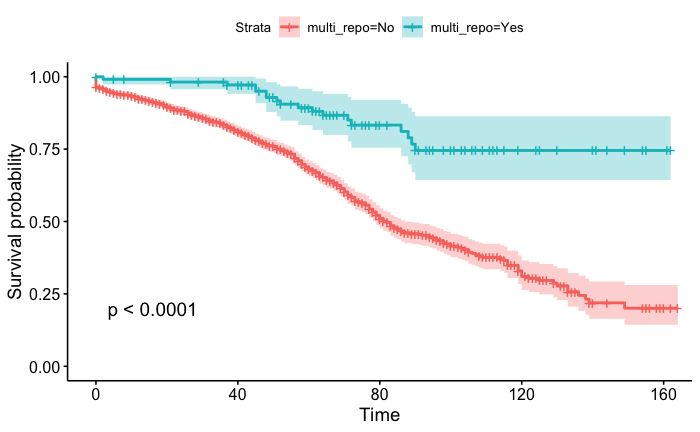
\includegraphics[width=0.45\textwidth]{multi_repo.png}
        \label{fig:multi repo}
    \end{subfigure}
    \begin{subfigure}   
        \centering 
        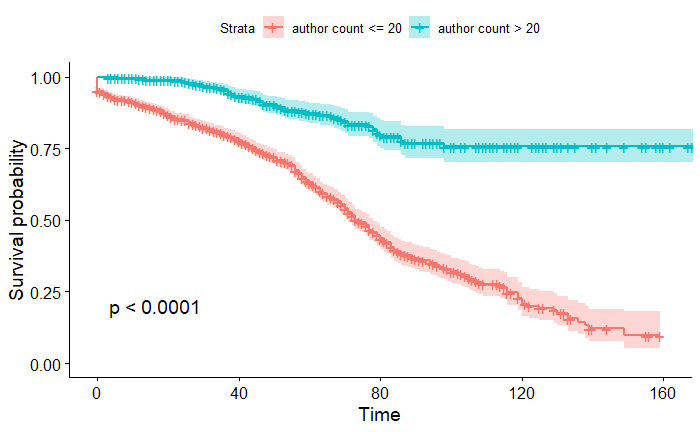
\includegraphics[width=0.45\textwidth]{img/author_count.png} 
        \label{fig:author count}
    \end{subfigure}
    \caption
    {\small KM curves of the python project data analyzed by major releases, host type, multiple repository hosting, and number of authors} 
    \label{fig:KM curves}
\end{figure*}

\begin{figure}[ht]
\centering
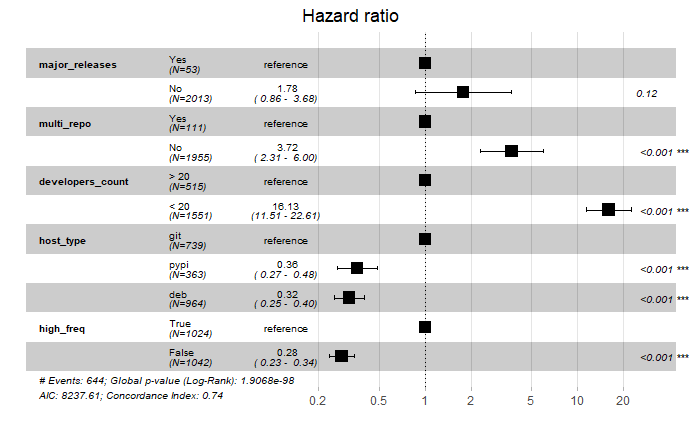
\includegraphics[scale=0.5]{cox-ratios.png}
\caption{The results of running the Cox Proportional hazards tool on the data. \keanu{we definitely want better descriptions for the images}}
\label{fig:Cox}
\end{figure}

\keanu{talk about significance and meaning of the KM and Cox results}

\keanu{As you can see in the Cox table summary, the numbers in each category are slightly different than the original study,
 we plan to look further into what has caused this difference in values}

\subsection{Revision Frequency Analysis}

\begin{figure}[H]
    \centering
    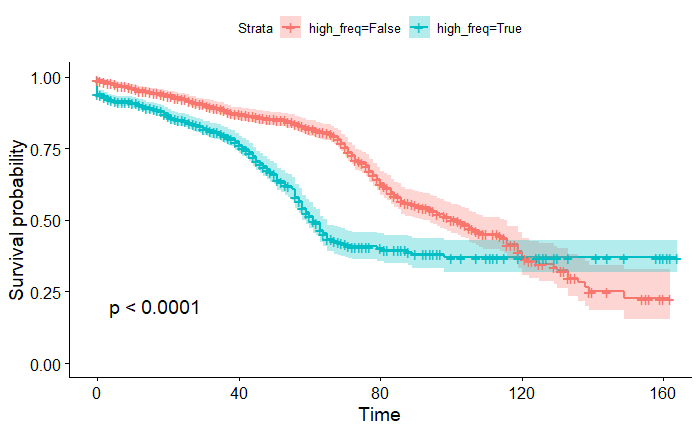
\includegraphics[scale=0.75]{commit_freq.png}
    \caption{KM curve for the data by revision frequency \keanu{need a better caption}}
    \label{fig:freq}
\end{figure}

\subsection{Bayesian Survival Analysis}

\begin{figure}[H]
    \centering
    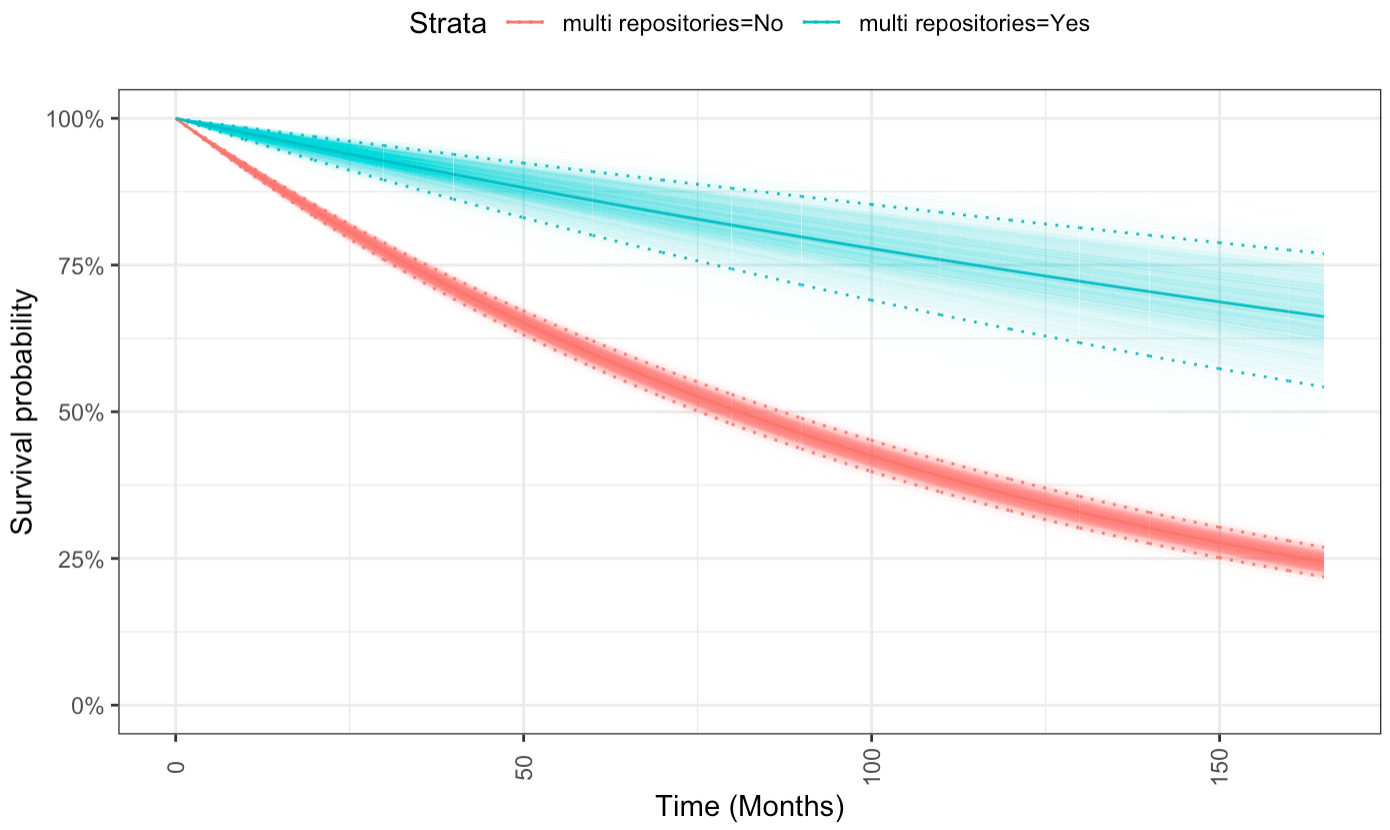
\includegraphics[scale=0.4]{multi_repo_bayes.png}
    \caption{Posterior survival functions of projects hosted on multiple repositories and projects hosted on a single repository}
    \label{fig:multi_repo_bayes}
\end{figure}

Shown in figure \ref{fig:multi_repo_bayes} are the posterior survival functions for projects host on multiple repositories versus those hosted on single repositories. The dotted lines represent the  2.5\% and 97.5\%
quantiles while the middle solid line represents the posterior mean of $\beta$ (the prior on the project attribute of interest). The remaining lines all represent valid posterior survival functions.

\section{Discussion} \label{discussion}

\subsection{Comparison of Analyses} \label{compare}

\keanu{We are not quite ready for a comparison yet}

\subsection{Limitations} \label{limit}

\subsubsection{Limitations of the Methods} \label{limit-methods}

The original paper \cite{ali2020cheating} and the MSR presentation given \cite{ali2020video} have contradicting methods of censoring.
The method discussed in the original paper was deemed superior and used in this paper.

Many details of the original paper's methods are left out for the sake of brevity.
This lead to assumptions being made when manipulating the data.
Hence, there are variations in the values retrieved compared to the original paper.
\keanu{NOTE: We are continuing to look into the possible causes of these inconsistencies. We will analyze our data-collection jupyter notebook and compare it with the end result of the R notebook to verify consistency between them before concluding it is an issue with the methods used}

% This following section is from the proposal and should be
% refined for the final report
Survival analysis methods such as the K-M estimator and the Cox Proportional-Hazards model have limitations of their own.
When applying the K-M estimator, it is common to use a log-rank test to test the significance between the two groups which are being compared.
The log-rank test only indicates whether or not the probability of survival is statistically significant between the two groups and is not able to provide any information about the size of the difference between the two groups \cite{stel2011kaplan}.
Additionally, the K-M estimator does not account for confounding factors \cite{stel2011kaplan}.
In more traditional uses of the K-M estimator, an example of a confounding factor could be the age of the study participants.
In the case of this study, there may be confounding factors such as the experience level of the developers or whether the developers received funding to work on the project.
Neither of these factors are represented in the data set.
The Cox Proportional-Hazards model is used with the assumption that, over the period of observation, the hazards within each group are proportional \cite{stel2011cox}.
If the assumption that the hazards within each group are proportional is not true, then the Cox Proportional-Hazards model will lead to incorrect estimates of the survival probability \cite{stel2011cox}. \keanu{we should assure the reader that it holds true in our case}

The Bayesian approach to survival analysis comes with its own limitations as well.
As pointed out by Renganathan, Bayesian survival analysis can be subjective as the analyst places their own bias into the model when selecting the prior distributions \cite{renganathan2016overview}.
In order to mitigate this bias, prior selection requires both epistemological and ontological reasoning. \keanu{We need to flesh out our reasoning more, probably written in the methods, but then perhaps referred to here}

\subsubsection{Limitations of the Data}

The data set in this study has been aggregated from multiple version control systems across the web over a large period of time.
As such, the data set is not fully reproducible, as pointed out by the original authors of the Software Heritage organization \cite{pietri2019software}.
Additionally, it cannot be ensured that the data contains a full history of the respective repositories.
The lack of certainty about the full history is because the repository admin can modify the history of revisions to suit their liking.
\keanu{add citation to perils of mining git}

There are inherent differences in the ways developers use the different hosting services \keanu{I have a strong intuition that this is the case, it looks like PyPi and debian don't have as much granularity compared to git and only show major releases, but I don't have anything to back this up, so maybe we can find something to cite for that}.
This could skew the results because it may be the case that services such as PyPi and Debian are primarily used to host major releases of a product.
This may hide information about the number of developers and the commit frequency.
Additionally, the potential confounding factors mentioned in section \ref{limit-methods} are not represented in this data set.

It may also be worth noting that this data is only for Python projects and that it is possible that different behaviours are associated with development in different languages.
Python is a relatively easy language to use, and can often be used for small tasks that are not maintained.
However, because this data set comprises popular projects, it is unlikely to contain projects that were used for a small task and discarded.

There was no clear method for determining whether a project was hosted in multiple repositories.
The only unique identifier for each project was a url, from which the project name was extracted using regular expressions.
This may have resulted in the extraction of inconsistent project names across host types.
The assumption is that each project that was hosted on multiple repositories would be given the exact same name, and that projects of the same name hosted on different services were indeed the same project (which may not always be the case).
Additionally, it is possible for users on Github to give their projects the exact same name as pre-existing projects created by other users.
However, this issue was accounted for in our analysis, but it is unclear whether Ali \emph{et al.} accounted for this.

The data contains a large portion of censored data.
This means that we did not observe the abandonment of most of the projects.
As data points are censored (denoted by the vertical tick marks in the KM curves), we have a smaller and smaller group of data points to study.
This means that the results towards the 165 month mark may be less representative.
This is to be expected with any SE study, as recent years have lead to an exponential increase in the number of OSS projects \keanu{find citation?}.


The data set contained many revisions (over 4 million) that were not associated with project URLs.
It is unclear how this happened.

% Not sure we need this
%\subsubsection{Replication Challenges}

\subsection{Related Work} \label{related}

Although the application of survival analysis is new to predicting the health of software repositories, several studies have attempted to analyze the health of open-source projects using different techniques. 
Xia \emph{et al.} \cite{xia2020predicting} applied DECART hyperparameter optimization to predict health indicators of open-source projects and observed that DECART reduced prediction errors of estimation algorithms by 10\%. 
Norick \emph{et al.} \cite{norick2010effects} analyzed open-source projects using code quality measures and observed no significant evidence that the number of committing developers affects software quality. 
Another study by Caivano \emph{et al.} \cite{caivano2021exploratory} investigated the spread and evolution of dead code by analyzing commit histories of open-source Java applications. 
They found that dead methods generally survive long, are rarely revived, and that a majority have been dead since their creation.

An application of survival analysis to software was a study by Samoladas \emph{et al.} \cite{samoladas2010survival} which predicted future development of FLOSS projects using project duration, application domain and the number of committers as predictors. 
The study calculated the probability of termination or continuation for FLOSS projects and quantified the benefit of adding more committers.

\subsection{Future Work} \label{future}

Increase the time frame of the study (the original paper could not do this because the paper was written in 2018).

Perform separate studies on each hosting service to remove variability in the way the services are utilized.

\section{Conclusion} \label{conclusion}

%%
%% The next two lines define the bibliography style to be used, and
%% the bibliography file.
\bibliographystyle{ACM-Reference-Format}
\bibliography{refs.bib}

%%
%% If your work has an appendix, this is the place to put it.
\appendix

\section{Artifacts} \label{artifacts}
Project Repository: \url{https://github.com/DerekRobin/CSC578B-Project}

Data Set: \url{https://annex.softwareheritage.org/public/dataset/graph/latest/popular-3k-python/sql/}

\end{document}
\endinput
